% %%%%%%%%%%%%%%%%%%%%%%%%%%%%%%%%%%%%%%%%%%%%%%%%%%%%%%%%%%%%%%%%%%%%%%%%%%%%%
\chapter{Neural Machine Translation}
\label{chap:nmt}
% %%%%%%%%%%%%%%%%%%%%%%%%%%%%%%%%%%%%%%%%%%%%%%%%%%%%%%%%%%%%%%%%%%%%%%%%%%%%%

\Ac{nmt} is the current state-of-the-art approach to \ac{mt}. As the name
suggests, \ac{nmt} systems use artificial neural networks to model the
translation. The specific types, or \emph{architectures}, of neural networks
used in an \ac{nmt} system vary across history, applications, or domains, but
all share a few common traits.

Neural networks are a mathematical model that works with real numbers. The
inputs and outputs to a neural network are real-valued vectors, the training
objective is a differentiable function, and the space of the parameters needs
to have a continuous gradient with respect to the loss function. Specific to
neural networks is the computation of the gradient by the
\emph{backpropagation} algorithm and the wide variety of optimization methods.

In Section \ref{sec:text-processing}, we explain how to adapt neural networks
to the discrete nature of the textual data. Perhaps the most common way is to
assign a real-valued vector to each word in the vocabulary. These
representations are usually trained along with the whole network end to end.

In \acs{nlp} tasks like sentence classification or language modeling, there is
only a single sequence on the input. In \ac{mt}, we have a source sentence on
the input and a target sentence on the output. To reflect this property, most
\ac{nmt} architectures have two components: an \emph{encoder} and a
\emph{decoder}. The encoder processes the input sentence and creates a hidden
representation. The decoder then accesses this hidden representation and
generates (or scores) the output sentence. When both components of the model
are trained end to end, this framework is sometimes referred to as
\emph{sequence-to-sequence learning}. We explore the encoder-decoder
architectures more closely in Section \ref{sec:encdec}.

Textual data are sequential, and the lengths of the sequences are
variable. Therefore, the use of feed-forward neural networks is not
suitable. Sequences can be processed by a number of network architectures,
namely \acp{cnn}, \acp{rnn}, or \acp{san}. All of those can be adapted for text
processing, and we will describe the latter two in more detail in Sections
\ref{sec:encdec:rnn} and \ref{sec:encdec:transformer}, respectively.

% Section about training: batching, optimization, multiple GPUs, ...
\ac{nmt} models are trained using large parallel corpora, by minimizing the
negative log-likelihood of the data.  Section \ref{sec:training} formalizes the
supervised training framework for translation models and summarizes the
training methodology, such as data processing, model initialization, and
optimization.

% Section about decoding
During training, sequence-to-sequence decoders usually run in the \emph{teacher
  forcing} mode -- for a given source sentence and its translation, the neural
network is trained to maximize the likelihood of the $i$-th target word on the
$i$-th position, conditioned on the $i-1$ previous words of the reference
sentence. During decoding, when this information is not available, the model is
conditioned on previously decoded outputs instead. More details on this
phenomenon and other practical considerations and techniques such as beam
search or ensembling are presented in Section \ref{sec:decoding}.

% alternative paragraph for Training section overview. Focus on batching and
% optimization instead of teacher forcing.

\Ac{mt} is evaluated by automatic metrics such as \acs{bleu} and by human
evaluation. This chapter concludes with a brief overview of the evaluation of
\ac{nmt} systems (Section \ref{sec:evaluation}).

% ------------------------------------------------------------------------------
\section{Processing Text with Neural Networks}
\label{sec:text-processing}
% ------------------------------------------------------------------------------

% Text are not numbers, NNs work with numbers
There are a number of problems that arise when we want to use neural networks
for text processing. First and foremost, neural networks are a mathematical
model that deals with real numbers, whereas language is discrete and has a
complex structure. Thus, we need to find ways to express textual data
numerically. Second, since language units (such as words, sentences, or
documents) come in various lengths, we need to use neural network models
designed for processing sequential data.

% One-hot representation are straightforward.
In this section, we begin with the representation of words. The most
straightforward and also the most common way to represent words in neural
networks is to have a list (a \emph{vocabulary}) of words $\mathcal{V}$ of size
$N$, where each word has a corresponding integer index $j$ pointing at it. Each
word $w$ at index $j$ in this list can be represented by a \emph{one-hot} vector
$x \in \{0,1\}^N$ where
%
\begin{equation} x_i =
\begin{cases} 1, & \text{if } i = j \\ 0, & \text{otherwise.}
\end{cases}
\end{equation}
%
% We call this vector the \emph{one-hot representation} of $w$.

% One-hot representation do not capture word roles in language.
Using one-hot representation helps us convert discrete words to numbers, but it
does not capture anything about the underlying linguistic structure.  For this
purpose, \emph{learned distributed feature vectors}, or \emph{word embeddings}
are used \citep{bengio2003neural, collobert-weston-2007-fast}. The idea is to
associate a real-valued vector with each word, so that representations of words
with similar roles in language are closer together in the assigned vector
space. \citet{mikolov-etal-2013-distributed} train these word embeddings using
the \emph{skip-gram} and \emph{continuous bag-of-words} objectives and find
that the resulting embeddings have interesting properties. For example,
arithmetic operations on embeddings can express word analogy.  In some \ac{nlp}
tasks, pre-trained embeddings can be used to greatly improve the model
performance on the end task. In contemporary \ac{nmt} research, the most
prevalent approach is to train the word embeddings end to end along with the
translation model.

% Word embedding layer is inserted to help.
We provide the model with the distributed representation of words using an
embedding layer as follows. For a given one-hot vector $x$ and a parameter
matrix $E$ called the \emph{embedding matrix}, we retrieve a single row that
corresponds to the vocabulary index of $x$ by multiplication $E x$.  The
embedding dimension is usually much lower than the size of the vocabulary (in
\ac{nmt}, the embedding dimension in state-of-the-art models is around 1,024).

% There are out-of-vocabulary tokens
A major drawback of having a fixed vocabulary is the fact that there will be
unseen words in the data. The following section lists methods that solve this
problem.


% -----------------------------------------------------------------------------
\subsection{Open Vocabulary Problem}
\label{subsec:openvoc}
% -----------------------------------------------------------------------------

A well-known characteristic of language is that it follows Zipf's law
\citep{zipf1949human}. As a result, in a large enough sample of text, there is
a huge amount of unique words or words occurring with low frequency. Such words
constitute a substantial part of the data and cannot be ignored.  Another issue
is that our training datasets do not contain all words that can occur in the
language. These \ac{oov} words usually also make up significant portions of the
validation and test data.

% Open vocabulary problem
The problem of rare and unseen words is also referred to as the \emph{open
  vocabulary} problem. Although some work in this direction exists
\citep{jean-etal-2015-using}, in neural networks for \ac{nlp}, it is difficult
to use very large vocabularies. The main reason is that the embedding layer and
the output projection layer would become too large for the computation to be
efficient.

% Most common solution
The most common solution of the open vocabulary problem is to use smaller units
than words \citep{sennrich-etal-2016-neural}. These \emph{subword} units can be
constructed in a smart way, such that frequent words are left intact, whereas
rare words are composed of more common strings of letters. In the following, we
describe three of the methods for subword segmentation. It is worth mentioning
that the research on character-level methods is still ongoing
\citep{chung-etal-2016-character,lee-etal-2017-fully,gao-etal-2020-character},
but as of the writing of this thesis, this approach did not yet outperform the
state-of-the-art subword segmentation.

% - - - - - - - - - - - - - - - - - - - - - - - - - - - - - - - - - - - - - - -
\paragraph{\acs{bpe}.}  \Acl{bpe} \glsunset{bpe} (\acs{bpe};
\citealp{sennrich-etal-2016-neural}) is an approach that tackles the open
vocabulary problem by splitting words into subword units.  The idea is to
devise a vocabulary of a predefined size such that any word can be composed
using the units from the vocabulary (with the exception of words containing
unknown characters). An additional requirement is for the vocabulary to contain
whole words that are frequent in the data, so only rare words are split into
more subwords. The \ac{bpe} method works with a vocabulary of merges, which
needs to be created by the \ac{bpe} training algorithm before it can be applied
on the data.

The \ac{bpe} training algorithm proceeds in iterations as follows.  At first,
all the tokens in the data are split into characters, and the vocabulary is
initialized with the list of the characters. To allow for later reconstruction
of the original text, a special end-of-word character is appended to each word.
Each iteration of the algorithm has three steps. First, the algorithm computes
the counts of pairs of consecutive symbols (bigrams) in the data (respecting
the word boundaries), and selects the most frequent pair. Second, the selected
bigram is merged and added to the vocabulary. Third, the new vocabulary is used
to segment the data again. These three steps are repeated until a predefined
number of merges are performed.  Note that in practice, the algorithm can be
implemented to work only with the frequency list of tokens, and not with the
whole training corpus, without loss of generality.

Once the \ac{bpe} merge list is created, it can be applied on the data by first
splitting the words in the data to characters, and then applying the learned
merges on the split words. Reconstruction of the original text can be done by
removing the spaces and then replacing the end-of-word characters with new
spaces.

% - - - - - - - - - - - - - - - - - - - - - - - - - - - - - - - - - - - - - - -
\paragraph{Wordpiece.} The wordpiece algorithm
\citep{schuster-nakajima-2012-japanese,wu2016google} shares the ideas of the
\ac{bpe} algorithm -- whole words are split into sequences of characters, which
are then merged according to a list of merges. Unlike the \ac{bpe}
segmentation, the wordpiece learning algorithm does not take the most frequent
bigram, but instead the pair with the largest pointwise mutual
information.
% \JH{They say they take the pair that maximizes the likelihood of the data,
% but then we would need to talk about language models first, and I guess it's
% the same thing.}

% - - - - - - - - - - - - - - - - - - - - - - - - - - - - - - - - - - - - - - -
\paragraph{SentencePiece.} More recently,
\citet{kudo-richardson-2018-sentencepiece} implemented SentencePiece, a toolkit
for subword segmentation using either \ac{bpe}, or a unigram language model
\citep{kudo-2018-subword}. It supports a number of features, such as sampling
and regularization by introducing noise on the source side. As opposed to BPEs
and wordpieces, SentencePiece does not require prior tokenization of the input
text, and unlike other methods its pre-tokenization allows to fully reconstruct
the original string. The Marian toolkit
\citep{junczys-dowmunt-etal-2018-marian} used in our experiments described in
Chapter \ref{chap:experiments} has built-in support for SentencePiece
tokenization and segmentation.


% ------------------------------------------------------------------------------
\section{Encoder-Decoder Framework}
\label{sec:encdec}
% ------------------------------------------------------------------------------

The contemporary \ac{nmt} models share a common framework where each model is
composed of two parts -- an \emph{encoder} and a \emph{decoder}. The encoder
reads the input sentence and processes it to generate an intermediate hidden
representation.  The decoder then uses this intermediate hidden representation
to produce the probability distributions over the output tokens.

The early \ac{nmt} models based on \acp{rnn} use the final encoder state as the
intermediate representation \citep{sutskever2014sequence}:
%
\begin{align}
  h_j &= \mathrm{RNN}_{\text{enc}}(x_j, h_{j-1}), \quad j \in
          \{0, 1, \ldots, T_x \} \\
  s_0 &= h_{T_x}
\end{align}
%
where $\mathbf{x}$ is the input sentence and $h_0$ is the initial hidden state,
usually set to $\mathbf{0}$. $T_x$ denotes the length of the input sentence.
Note that the input words are represented as their embeddings.
\citet{sutskever2014sequence} do not use subword segmentation and instead
reserve a special \ac{oov} token for unseen words.

The decoder is initialized with the state $s_0$ and runs the second \ac{rnn}:
\begin{equation} s_i = \mathrm{RNN}_{\text{dec}}(y_{i-1}, s_{i-1})
\end{equation}
%
where $y_{i-1}$ is the preceding word in the reference output sentence (during
training), with $y_0$ being a special symbol that expresses the start of a
sequence (denoted \texttt{<s>}).

While recurrent neural networks are not used as the underlying model in most of
the current research anymore, the encoder-decoder framework is independent of
the actual neural network structure and the concept is still used as the main
approach for designing sequence-to-sequence models.

In this section, we introduce the two most notable encoder-decoder
architectures. The first is based on \acp{rnn} and became the first neural
architecture to outperform statistical \ac{mt} models. The second architecture,
called \emph{Transformer}, is based on self-attentive networks and is the best
performing architecture for many \ac{nlp} tasks today.


% -----------------------------------------------------------------------------
\subsection{Recurrent Neural Networks}
\label{sec:encdec:rnn}
% -----------------------------------------------------------------------------

The invention of \acp{rnn} \citep{elman1990finding} allowed processing of
sequential data by neural networks. \Acp{rnn} process the sequence one item at
a time, chaining consecutive steps with recurrence connections.

In the early stages of the \ac{rnn} development, a single hidden layer of the
network was altered to take into account the output of itself from the previous
time step:

%\begin{equation} % h_t = f(x_t, h_{t-1})
%\end{equation}
%
%\noindent %where $f$ is usually a non-linear projection:

\begin{equation} h_t = \tanh ( W x_t + U h_{t-1} + b_h ) \label{eq:vanilla-rnn}
\end{equation}

\noindent where $W \in \mathbb{R}^{m \times n}$,
$U \in \mathbb{R}^{n \times n}$, $b_h \in \mathbb{R}^{n}$ are trainable
parameters, $x_t \in \mathbb{R}^{m}$ is the \ac{rnn} input, and
$h_{t-1} \in \mathbb{R}^{n}$ is the previous hidden state.

However, this version of \acp{rnn} suffers from the \emph{vanishing gradient
  problem}. During backpropagation, the gradients are multiplied by the
derivative of the hyperbolic tangent, which is always less than or equal to
one. In long sequences, the learning signal over distant parts of the sequence
therefore has almost no effect on the training. Due to this fact, the network
manifests poor performance in handling long-range dependencies.

There have been several approaches to combat the vanishing gradient problem.
The most prevailing types of \ac{rnn} architectures in \ac{nmt} are \ac{lstm}
networks and \ac{gru} networks.

% - - - - - - - - - - - - - - - - - - - - - - - - - - - - - - - - - - - - - - -
\paragraph{\acs{lstm}.} \acl{lstm} networks
\citep{hochreiter1997long,gers2000learning} introduce gating mechanisms and a
concept of \emph{information highway}, which ensures that only linear
operations are applied on the states in the recurrent chain. A gating mechanism
is an operation that computes a number between 0 and 1, which we refer to as a
\emph{gate value}.  The output of the operation is the input multiplied by the
gate value.

Given a current time step $t$, input $x_t \in \mathbb{R}^m$, and previous
hidden states $h_{t-1}, C_{t-1} \in \mathbb{R}^n$, \ac{lstm} networks proceed
as follows:
%
\begin{align}
  f_t &= \sigma\left(W_f x_t + U_f h_{t-1} + b_f\right) \label{eq:lstm-forget-gate} \\
  i_t &= \sigma\left(W_i x_t + U_i h_{t-1} + b_i\right) \label{eq:lstm-input-gate} \\
  o_t &= \sigma\left(W_o x_t + U_o h_{t-1} + b_o\right) \label{eq:lstm-output-gate} \\
  \tilde{C}_t &= \tanh \left( W_c x_t + U_c h_{t-1} + b_c \right) \label{eq:lstm-candidate} \\
  C_t &= f_t \odot C_{t-1} + i_t \odot \tilde{C}_t \label{eq:lstm-information-highway} \\
  h_t &= o_t \odot \tanh C_t \label{eq:lstm-hidden-state}
\end{align}
%
where $W_f, W_i, W_o, W_c \in \mathbb{R}^{n \times m}, U_f, U_i, U_o, U_c \in
\mathbb{R}^{n \times n}, b_f, b_i, b_o, b_c \in \mathbb{R}^n$ are trainable
parameters, $\sigma$ is the logistic function, and $\odot$ represents
element-wise multiplication. The states $h_t$ and $C_t$ are also called public
and private hidden states, respectively. The intermediate value $\tilde{C}_t$ is
called the candidate state.

The three gates in the \ac{lstm} network are called the \emph{forget gate}, the
\emph{input gate}, and the \emph{output gate}. The forget gate (Eq.
\ref{eq:lstm-forget-gate}) controls how much of the information flows from the
previous private hidden state $C_{t-1}$ to the current private state (Eq.
\ref{eq:lstm-information-highway}). The input gate (Eq.
\ref{eq:lstm-input-gate}) controls the amount of information received from the
candidate state. Finally, the output gate (Eq. \ref{eq:lstm-output-gate})
decides which portion of the currently computed private hidden state is
transferred to the current public hidden state
(Eq. \ref{eq:lstm-output-gate}). Note that the values of the gates are computed
in the same way, but with different parameters.

The original recurrence relation from Equation \ref{eq:vanilla-rnn} is expressed
by Equation \ref{eq:lstm-candidate}, where the new candidate state is
computed. The transfer of information from the previous private state and the
current candidate state is done in Equation
\ref{eq:lstm-information-highway}. Note that with respect to the states from the
preceding steps, the previous state is only multiplied by a constant. This
constitutes the information highway that allows propagating the gradients over
long distances in the sequence.

% - - - - - - - - - - - - - - - - - - - - - - - - - - - - - - - - - - - - - - -
\paragraph{\acs{gru}.} \acl{gru} networks \citep{cho-etal-2014-properties} are
an alternative to \acp{lstm}. Instead of four sets of parameter matrices,
\acp{gru} need only three, while maintaining the theoretical strength. Unlike
\acp{lstm}, \acp{gru} use only a single hidden state in the recurrence
relations.

Given the time step $t$, the input $x_t \in \mathbb{R}^m$, and the previous
hidden state $h_{t-1} \in \mathbb{R}^n$, the \ac{gru} step is defined as
follows:
%
\begin{align}
  r_t &= \sigma\left(W_r x_t + U_r h_{t-1} + b_r\right) \label{eq:gru-reset-gate} \\
  z_t &= \sigma\left(W_z x_t + U_z h_{t-1} + b_z\right) \label{eq:gru-update-gate} \\
  \tilde{h}_t &= \tanh \left(W x_t + U \left( r_t \odot h_{t-1} \right) + b \right) \label{eq:gru-candidate} \\
  h_t &= (1 - z_t) \odot h_{t-1} + z_t \odot \tilde{h}_t \label{eq:gru-hidden-state}
\end{align}
%
where $W, W_z, W_r \in \mathbb{R}^{n\times m}$,
$U, U_z, U_r \in \mathbb{R}^{n \times n}$, and $b, b_z, b_r \in \mathbb{R}^n$
are trainable parameters.

The two gates in \ac{gru} networks are called the \emph{reset gate} and the
\emph{update gate}.  The reset gate (Eq. \ref{eq:gru-reset-gate}) determines
how much information from the previous state is preserved and is applied in the
recurrence relation for computing the candidate
(Eq. \ref{eq:gru-candidate}). The update gate (Eq.  \ref{eq:gru-update-gate})
controls the merging of the previous state with the candidate state in Equation
\ref{eq:gru-hidden-state}. Note that the information highway concept is
expressed by this equation.

% - - - - - - - - - - - - - - - - - - - - - - - - - - - - - - - - - - - - - - -
\paragraph{Bidirectional RNNs.} There is a bidirectional variant of \acp{rnn}
that can be applied to any of the flavors of \acp{rnn} discussed above. When
the whole input sequence is known, we can apply an \ac{rnn} in both directions
separately and then concatenate the states from the corresponding positions:
%
\begin{align}
  \overrightarrow{h}_t &= \overrightarrow{\mathrm{RNN}}(x_{t-1}, \overrightarrow{h}_{t-1}) \\
  \overleftarrow{h}_t &= \overleftarrow{\mathrm{RNN}}(x_{t+1}, \overleftarrow{h}_{t+1}) \\
  h_t &= \left[ \begin{matrix} \overrightarrow{h}_t \\ \overleftarrow{h}_t \end{matrix} \right]
\end{align}

% - - - - - - - - - - - - - - - - - - - - - - - - - - - - - - - - - - - - - - -
\paragraph{Attention Mechanism.} Another important concept introduced as part
of \ac{rnn}-based \ac{nmt} models is the \emph{attention mechanism}
\citep{bahdanau2014neural,luong-etal-2015-effective}.

The problem with the encoder-decoder framework as described in the previous
section is that there is an information bottleneck between the encoder and the
decoder. All the information from the source sentence needs to be compressed
into a single hidden state vector $s_0$.

The attention mechanism enables the decoder to access the information stored in
the encoder hidden states rather than relying only on the value of the initial
state.  Formally, based on a current decoder step $s_i$, the attention mechanism
computes a local \emph{context vector} as a weighted average of the encoder
states:
%
\begin{align}
  % attn energies
  e_{ij} &= v_a^\top \tanh (W_a s_{i-1} + U_a h_j + b_a) + b', \label{eq:attn-energies} \\
  % attn distro
  \alpha_{ij} &= \frac{\exp(e_{ij})}{\sum_{k=1}^{T_x}\exp(e_{ik})}, \\
  %
  % \softmax_{j \in 1, 2, \ldots, T_x } & = & e_{ij} \\
  % context vector
  c_i &= \sum_{j=1}^{T_x} \alpha_{ij} h_j.
\end{align}
%
In the first step, the \emph{attention energies} are computed for every encoder
hidden state using a single-hidden-layer feed-forward network parameterized by
$W_a \in \mathbb{R}^{n' \times n}$, $U_a \in \mathbb{R}^{n' \times 2n}$ (in a
bidirectional network), $b_a \in \mathbb{R}^{n'}$, $v_a \in \mathbb{R}^{n'}$,
and $b' \in \mathbb{R}$ where $n'$ is the dimension of the hidden layer. Next,
the attention energies are normalized using the softmax function into the
\emph{attention distribution}.  Finally, the context vector is computed as a
weighted sum of the encoder states $h_0,\ldots, h_{T_x}$, using the attention
distribution values as weights.

The concept of attention can be viewed as a soft-lookup function over an
associative memory. Given a \emph{query}, which is the decoder state in a given
time step, we use a similarity metric over a set of \emph{keys}. We then
normalize the similarities and use them as weights in the weighted sum of the
\emph{values} associated with the corresponding keys. In this case, the sets of
attention keys and values are equal to the encoder hidden states $h_j$. The
similarity metric is defined in Equation \ref{eq:attn-energies}.

% - - - - - - - - - - - - - - - - - - - - - - - - - - - - - - - - - - - - - - -
\paragraph{Deep \acp{rnn}.} Some NMT architectures based on \acp{rnn} use
multiple recurrent layers \citep{miceli-barone-etal-2017-deep,wu2016google}. In
deep \acp{rnn}, each layer is a recurrent network. The inputs of the second and
each layer onwards are the outputs of the preceding layer. The output of the
entire deep \ac{rnn} is the output of the last layer.

In deep \acp{rnn}, there are a few settings to consider.
%\JH{tell me more -- if not more, make this a layernorm paragraph}
%
% \JH{first layer norm paragraph should give better motivation, last paragraph
%   should provide some insight to the formulas.}
To improve the convergence speed of the deep models and to stabilize the
\ac{rnn} hidden state dynamics across layers, \emph{layer normalization}
\citep{ba2016layer} is often employed. For layer $l$ and its output states
%$h_1^l, \ldots h_{T_x}^l$, $h_i^l \in \mathbb{R}^n$,
$\mathbf{h}^l \in \mathbb{R}^{T_x \times n}$, we compute:
%
\begin{align}
  \mu^l &= \frac{1}{nT_x} \sum_{i=1}^{T_x}\sum_{j=1}^n h^l_{ij} \\
  \sigma^l &= \sqrt{\frac{1}{nT_x} \sum_{i=1}^{T_x}\sum_{j=1}^n (h^l_{ij} - \mu^l)^2} \\
  \bar{\mathbf{h}}^l &= \frac{\mathbf{h}^l - \mu^l}{\sigma^l} \odot \gamma^l + \beta^l
\end{align}
%
where $\mu^l$ and $\sigma^l$ are the mean and standard deviation of the output
state values, $\gamma^l, \beta^l \in \mathbb{R}^{T_x \times n}$ are learnable
\emph{gain} and \emph{bias} parameters, and $\odot$ denotes element-wise
multiplication. Normalized states $\bar{\mathbf{h}}^l$ are then used as input
to the $(l+1)$-th layer of the network instead.

Another common technique in multilayer \acp{rnn} is to tie the vector spaces of
the \ac{rnn} states on different layers with residual connections. In such
networks, the input to the $(l+1)$-th layer is the sum of the output of the
$l$-th layer with its input.


% -----------------------------------------------------------------------------
\subsection{Transformer Model}
\label{sec:encdec:transformer}
% -----------------------------------------------------------------------------

One of the disadvantages of RNN-based models is the sequential nature of the
recurrence relation. A few models have been proposed to remove the recurrence,
thus allowing for simultaneous computation across time steps, at least at the
training time. Most notably, these models include convolutional architectures
\citep{gehring2017convolutional}, and the current state-of-the-art
architecture, the \emph{Transformer} model \citep{vaswani2017attention}.

Instead of recurrence relations, the Transformer model uses
\emph{self-attention} layers, stacked into a deep network. The states in each
layer can be computed independently on each other, which leads to training
speed improvements. We follow with a detailed description of the Transformer
model components, illustrated in Figure \ref{fig:transformer}.

\begin{figure}
  \centering
  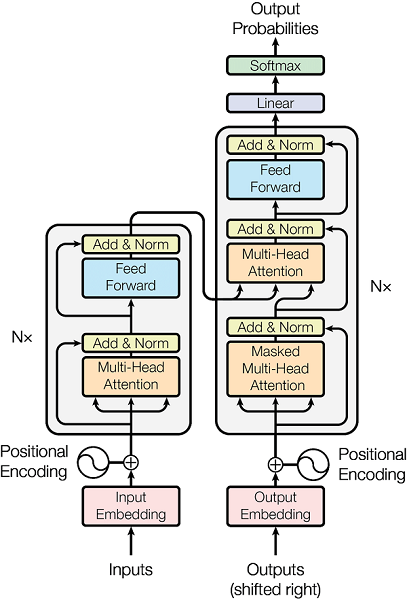
\includegraphics[width=9cm]{img/transformer.png}

  \caption{The overall schema of the Transformer model. The inputs are summed
    with positional encodings. The encoder processes the input in $N$ stack
    layers. Each encoder layer consists of self-attention and feed-forward
    sub-layer. Layers are interconnected with residual connections and layer
    normalization is applied on the output of each layer. The decoder stack
    uses three sub-layers, where the additional cross-attention layer attends
    to the encoder output. We show the original image from
    \citet{vaswani2017attention}, Figure 1.}
  \label{fig:transformer}
\end{figure}

% - - - - - - - - - - - - - - - - - - - - - - - - - - - - - - - - - - - - - - -
\paragraph{Positional Encoding.} Since self attention is a commutative
operation, the ordering of the input tokens needs to be modeled explicitly.
The standard technique is to use sinusoidal encodings, as proposed in the
original paper. Positional encoding is a vector of the same dimension as the
word embedding, which is computed using the position of the word on the input.
The $2i$-th and $(2i+1)$-th elements of the positional encoding of word on
position $j$ is computed as follows:
%
\begin{equation}
  \begin{split}
    E_{\text{pos}}(j, 2i) &= \sin(j / 10000^{2i/d}) \\
    E_{\text{pos}}(j, 2i + 1) &= \cos(j / 10000^{2i/d})
  \end{split} \label{eq:positional-encoding}
\end{equation}
%
where $d$ is the \emph{model dimension}. This number is equal to the dimension
of the word embeddings. Before the network processes an input word $w_i$, the
positional encodings are added to the word embeddings:
\begin{equation}
  E(w_i) = E(w) + E_{\text{pos}}(i)
\end{equation}

% - - - - - - - - - - - - - - - - - - - - - - - - - - - - - - - - - - - - - - -
\paragraph{Self-Attention.} The key component of the Transformer model is
self-attention. As the name suggests, self-attention is run with the same set
of states used as queries, keys, and values. The scaled dot product is used as
the similarity metric, so the attention itself does not use any trainable
parameters. Formally, self-attention is defined as a function:
%
\begin{equation}
  \mathcal{A}(Q,K,V) = \softmax \left( \frac{QK^\top}{\sqrt{d}} \right) V
  \label{eq:scaled-dot-product}
\end{equation}
%
where the values $Q, K, V \in \mathbb{R}^{T \times d}$ ($T$ being the sequence
length) are computed from the same input, usually using a linear projection.

Self-attention sub-layers are used both in the encoder and the decoder. Because
the decoder is autoregressive, the self-attention module must be limited to
attend only to the preceding states (so that the model does not ``glance into
the future''). This is implemented by applying a triangular mask (also
\emph{causal mask}) on the attention query and key matrix, hence the name
\emph{masked self-attetnion}.

% - - - - - - - - - - - - - - - - - - - - - - - - - - - - - - - - - - - - - - -
\paragraph{Multi-Head Attention.} Instead of running a single self-attention
per layer, the model structure is enriched by splitting the self-attention into
multiple \emph{heads}. First, each state is projected into $h$ triples of
queries, keys, and values. Then, self-attention is computed on each triple.
Finally, the self-attention outputs are mixed together into a single output
sequence:
%
\begin{equation}
  \mathcal{A}^h(Q, K, V) = \sum_{i=1}^h C_i W_i^O \\
\end{equation}
%
where $W_i^O \in \mathbb{R}^{d_h \times d}$ is a parameter matrix used to
project the outputs from the individual attention heads into a single output,
and
%
\begin{equation}
  C_i = \mathcal{A}(QW_i^Q, KW_i^K, VW_i^V)
\end{equation}
where $W_i^Q, W_i^K, W_i^V \in \mathbb{R}^{d \times d_h}$ are trainable
matrices that project the states to inputs for the $i$-th attention head
(defined in Equation \ref{eq:scaled-dot-product}). In self-attention,
$Q = K = V \in \mathbb{R}^{T \times d}$ is the set of $T$ states of the current
layer.

% - - - - - - - - - - - - - - - - - - - - - - - - - - - - - - - - - - - - - - -
\paragraph{Cross-Attention.} Each Transformer encoder layer consists of a
self-attention and a feed-forward sub-layer. The decoder inserts an
\emph{encoder-decoder attention} (or \emph{cross-attention}) layer.  The
cross-attention layer functions exactly like the self-attention layer, but the
queries $Q$ are the decoder states (i.e. the output of the preceding
self-attention), and the keys and values $K = V$ correspond to the encoder
output states.

% - - - - - - - - - - - - - - - - - - - - - - - - - - - - - - - - - - - - - - -
\paragraph{Feed-Forward Layer.} Each Transformer layer consists
of self-attention, optionally a cross-attention, followed by a feed-forward
network. This feed-forward network uses the same parameters for all positions
along the state sequence. The network takes a state $x$ and feeds it through a
single hidden layer with a ReLU activation:

\begin{equation}
  \mathcal{F}(x) = \max(0, W_1^Fx + b_1^F)W_2^F + b_2^F
\end{equation}
where $W_1^F \in \mathbb{R}^{d \times d_f}$, $b_1 \in \mathbb{R}^{d_f}$,
$W_2^F \in \mathbb{R}^{d_f \times d}$, and $b_2^F \in \mathbb{R}^d$ are the
weight and bias parameters of the feed-forward network $\mathcal{F}$, and $d_f$
is the dimension of the hidden state.

% - - - - - - - - - - - - - - - - - - - - - - - - - - - - - - - - - - - - - - -
\paragraph{Residual Connections and Layer Normalization.} As a post-processing
step, the output of each sub-layer is connected with the output of the previous
sub-layer with residual connections. Similarly to the \acs{rnn}-based deep
architectures, layer normalization is used in combination, which ties all
states in the sub-layer stack into a shared vector space.

% - - - - - - - - - - - - - - - - - - - - - - - - - - - - - - - - - - - - - - -
\paragraph{Output Projection.} The states of the last decoder layer are
projected to the size of the vocabulary and are interpreted as unnormalized
probability distributions over the output tokens. When a probability
distribution is needed (during training or beam search decoding), the scores
are normalized using the softmax function:
%
\begin{equation}
  p(y_t | y_{<t}, x, \theta) = \softmax( W^S s_t + b^S )
\end{equation}
%
where $W^S \in \mathbb{R}^{d \times |\mathcal{V}|}$,
$b \in \mathbb{R}^{|\mathcal{V}|}$ are the output projection parameters, $s_t$
is the $t$-th state in the last decoder layer, and $\theta$ is the set of model
parameters. Note that the probability of the $t$-th output token $y_t$ is
conditioned on the preceding tokens $y_{<t}$ because of the causal mask in the
decoder self-attention. In the Transformer model, it is possible to tie the
values of the output projection matrix with the transposed embedding
matrix. This reduces the number of model parameters and can have advantages
over separate input and output projection matrices when using a shared
source--target vocabulary.

To compute the probability distribution of the whole target sentence $y$ given
the input sentence $x$, the distributions from all time steps are multiplied
together:
%
\begin{equation}
  p(y|x) = \prod_{t=1}^{T_y}p(y_t|y_{<t},x,\theta)
  \label{eq:output-distribution}
\end{equation}
%
where $T_y \in \mathbb{R}$ is the length of the target sentence, $y_{<t}$ are
the previously decoded words.

% - - - - - - - - - - - - - - - - - - - - - - - - - - - - - - - - - - - - - - -
\paragraph{Model Hyperparameters.} The parameters that control the model size
are the model dimension $d$, the number of attention heads $h$, the dimension
of the feed-forward hidden layer $d_f$, and the number of Transformer layers in
the encoder and decoder stack. Note that the dimension of keys and values in a
single attention head $d_h$ is commonly set to be $d / h$, but can be
customized as well.  As a regularization, dropout \citep{srivastava2014dropout}
is applied with rate $P_d$ to the output of each sub-layer before
normalization.

The authors of the architecture propose two presets for these parameters, named
\emph{base} and \emph{big}. Table~\ref{tab:transformer-hyperparams} shows the
hyperparameter values for these two settings.

\begin{table}
  \centering
  \begin{tabular}{lrrrrrr}
    \toprule
      & \# of layers &  $d$  &  $h$  & $d_h$ & $d_f$ & $P_d$ \\
    \midrule
    Transformer base  & 6 &  512  & 8 & 64 &  2,048 & 0.1 \\
    Transformer big  & 6 &  1,024  & 16 & 64 &  4,096 & 0.3 \\
    \bottomrule
  \end{tabular}
  \caption{The hyperparameter values for Transformer base and big variants.}%
  \label{tab:transformer-hyperparams}
\end{table}


% ------------------------------------------------------------------------------
\section{Training}
\label{sec:training}
% ------------------------------------------------------------------------------

Training of \ac{nmt} models is usually done under \emph{supervised} conditions,
using a dataset of parallel sentences. The size of the available data varies
greatly with different language pairs. Although there is no formal definition,
a language pair for which less than a million sentence pairs are available is
usually referred to as \emph{low-resource}. For many languages, even a million
sentences is a very large number compared to what is actually available. Data
quality is also a factor. For example, when the only available data is crawled
from the web, data cleaning can filter out a major part of the corpus. However,
in this thesis, we focus on language pairs where the data size is not a major
issue.
% and we simulate the low-resource scenario using Romanian-English translation.

Translation models are trained by minimizing the loss function, usually
expressed by cross entropy between the output distribution and the one-hot
distribution that assigns zero probabilities to all but the correct target
word. Assuming that $y_i$ is the correct target word at position $i$,
$p_{\text{ref}}$ is the one-hot distribution, and $p$ is the distribution
predicted by the model, we have the following:
%
\begin{equation}
  \begin{split}
    H(p_{\text{ref}}, p) &=  - \sum_{w \in \mathcal{V}} p_{\text{ref}}(w) \log p(w) = \\
    &=  - \log p(y_i)
  \end{split}
\end{equation}
%
where $\mathcal{V}$ is the vocabulary. Note that in autoregressive models, the
output distributions $p$ and $p_{\text{ref}}$ are conditioned on the preceding
target words.

Given model parameters $\theta$, the word-level cross entropy is summed across
the sentence pairs in the data $D$ to obtain the negative log-likelihood of the
dataset $J(\theta)$:
%
\begin{equation}
  \begin{split}
  J(\theta) &= - \sum_{(x, y) \in D} \sum_{i = 1}^{T_y} \log p(y_i | x, y_{<i}, \theta) \\
  &= - \sum_{(x, y) \in D} \log p(y | x, \theta)
  \end{split} \label{eq:loss}
\end{equation}
%
where $y_{<i}$ denote the target prefix and $T_{y}$ is the length of the target
sentence $y$. The probability of a sentence can be reformulated using the chain
rule.

The goal of training is to find parameters $\theta^*$ that minimize the cost
function defined above:
\begin{equation}
  \theta^* = \argmin_{\theta}J(\theta)
\end{equation}


% - - - - - - - - - - - - - - - - - - - - - - - - - - - - - - - - - - - - - - -
\paragraph{Teacher Forcing.}
Note that in the equations above, the probability distributions are conditioned
on the reference target prefix, rather than the model output. This technique is
known as \emph{teacher forcing} and is essential for the convergence of
training. When the model is exposed to its own outputs from the start of the
training, it is very likely that it will fail to converge.

Teacher forcing, however, brings along a problem called \emph{exposure bias}:
the model is never exposed to its own errors, which makes it less robust
against them.

Methods have been proposed to address this issue, including a curriculum
learning approach which gradually replaces teacher forcing with the model
predictions \citep{bengio2015scheduled}. Other methods focus on sequence-level
training or beam search optimization methods, mostly based on reinforcement
learning \citep{williams1992simple, wiseman-rush-2016-sequence,
  daume2009search, ranzato2016sequence}. However, none of these methods has
been widely adopted, and current models are believed to be capable of
recovering from their errors, despite being explicitly trained to do so.

% - - - - - - - - - - - - - - - - - - - - - - - - - - - - - - - - - - - - - - -
%\paragraph{RNNs vs Transformer Training.} A significant difference in training
%\acp{rnn} and the Transformer model is


% -----------------------------------------------------------------------------
\subsection{Training Methodology}
\label{sec:training:methodology}
% -----------------------------------------------------------------------------

In this section, we go through common techniques for successful training of
\ac{nmt} models. These include data cleaning and augmentation methods,
optimization settings, and hardware considerations.

% - - - - - - - - - - - - - - - - - - - - - - - - - - - - - - - - - - - - - - -
\paragraph{Data Cleaning.} With a few exceptions for high-resource languages,
the training data is usually acquired from the Web. Depending on the data
source and the extraction technique, there is a level of noise present in the
data. In many cases, it is necessary to consider data cleaning before training
any models.

The basic data cleaning techniques are rule-based and include language
identification, and filtering sentence pairs with odd characters or length
ratios. Deduplication may be considered, but might be harmful when it removes
short sentences which appear commonly in the given language. For example, if
the English sentences ``Thank you'' and ``Thank you xxx'' both appear in the
data as translations of the Czech ``Děkuji'', they might get the same
probabilities when deduplication is used. Without deduplication, the frequency
of the correct translation would be much higher in the training data, but other
problems may arise, especially in data crawled from the Web, where there are
many repeated snippets from page headers or footers which do not occur
naturally so often.

An advanced data cleaning technique is dual conditional cross-entropy filtering
\citep{junczys-dowmunt-2018-dual}. Using two translation models trained on
clean data in opposite directions, each sentence pair is scored according to
the cross entropies assigned by the translation models to the sentence
pair. When the cross entropies differ or when both cross entropy scores are
high, the score is low. When the cross entropies are similar and are low, the
score is high. After scoring, low-scoring sentence pairs are removed from the
data using an empirically set threshold. Formally, each sentence pair $(x,y)$
is scored with the opposite models $A$ and $B$ according to the following
formula:
%
\begin{equation}
  s = |H_A(y|x) - H_B(x|y)| + \frac{1}{2} (H_A(y|x) + H_B{x|y})
\end{equation}
where $H_A$ and $H_B$ are the cross entropies of the two models, normalized
over words:
%
\begin{equation}
  H_A(y|x) = - \frac{1}{T_y} \log p(y|x)
\end{equation}
and similarly for $H_B(x|y)$.

% - - - - - - - - - - - - - - - - - - - - - - - - - - - - - - - - - - - - - - -
\paragraph{Data Augmentation.} The size of the training data is a key factor in
modeling performance. In rare cases of high-resource languages, there is enough
parallel data available to train a decent translation model. But even for these
languages, data augmentation methods, namely \emph{backtranslation}, are used
to create bigger data and therefore to improve the model performance.

Backtranslation is a simple technique for incorporating target-side monolingual
data in a translation model
\citep{bojar-tamchyna-2011-improving,sennrich-etal-2016-improving}. For a given
translation direction, we first translate the monolingual data from the target
language to the source language using a previously trained model. Then, we mix
the synthetic source-language data along with the authentic target-language
data into our training corpus. When the parallel-to-monolingual data size ratio
is not balanced, one can consider oversampling the smaller part of the corpus
to mitigate this. Recently, \citet{caswell-etal-2019-tagged} showed that
labeling the synthetic data with a special token improves the translation
quality. As pointed out by \citet{marie-etal-2020-tagged}, this helps because
the model is less prone to overfitting to this type of data.

\emph{Knowledge distillation} \citep{kim-rush-2016-sequence} is another data
augmentation technique. Unlike backtranslation, knowledge distillation is used
mainly to improve the efficiency of the model, both in terms of memory and
speed. Also, we use synthetic target-language data. In the simplest setting, we
use a well-trained and large \emph{teacher} model to translate its own training
data. Then, we train a smaller (and therefore faster and smaller)
\emph{student} model on the data generated by the teacher model. This technique
shows that for a small sacrifice in translation quality, we can get interesting
improvements in terms of speed, which is useful for deploying the models in a
limited environment, such as a mobile device.

% - - - - - - - - - - - - - - - - - - - - - - - - - - - - - - - - - - - - - - -
\paragraph{Batching.} In Equation \ref{eq:loss}, the loss function $J(\theta)$
is defined as a sum of sequence-level losses over dataset $D$. We use the
gradient descent algorithm to find the parameters $\theta^*$ with the minimum
loss value. The algorithm proceeds in iterations, updating the parameters using
current gradients.  However, the exact computation of the gradient is
inefficient because it requires a pass through the whole dataset. Therefore, we
estimate the gradient on a small sample of the training data, called a
\emph{mini batch}, or simply a batch. This method is called
\emph{\ac{sgd}}.\footnote{Some sources use the term \emph{mini-batch gradient
    descent}, to distinguish from methods that perform the update for each
  example.}

The size of a mini batch is an important parameter, and its value can have a
large impact on the training convergence. Bigger batches provide better
gradient estimates, but require more memory, which is a concern when using a
GPU.

Because the data gets split into batches that serve as random samples of the
data, a suitable data shuffling strategy should be considered. If we regard the
dataset as a collection of sentences (as opposed to documents, for example),
shuffling the sentences in the whole dataset before training (or before each
\emph{epoch}, i.e. a pass over the training data) is in most cases sufficient.

Another aspect of batching is how efficiently we use the memory allocated for
the batch with respect to the maximum sentence length. The batches are
represented as matrices, where each row corresponds to a sentence and each
column corresponds to a token position in the sentence. Sentences shorter than
the longest sentence in the batch are padded to the maximum length. If the
overall amount of padding used in a batch is large, the optimization step takes
longer. Therefore, we try to use batches of sentences with similar lengths. A
possible implementation is to load a number of batches beforehand, sort the
sentences by length, and then re-batch the sorted list of sentences. In the
literature, this technique is called \emph{bucketing}.

In some cases, it is possible to delay the parameter update for a number of
batches. For example, large models tend to fit into a GPU memory only with a
small batch size. In such cases, we might choose to aggregate the gradients
over multiple batches to simulate a larger batch size. A similar strategy can
be applied when the training uses multiple GPUs.

% - - - - - - - - - - - - - - - - - - - - - - - - - - - - - - - - - - - - - - -
\paragraph{Curriculum Training.} The ordering of the batches in training -- the
\emph{curriculum} -- influences both the training process (see bucketing above)
and the actual performance of the trained
model. \citet{kocmi-bojar-2017-curriculum} experiment with various curriculum
scenarios such as starting training on the shorter sentences and gradually
including more complex ones, which has been shown to somewhat improve the final
model. \citet{popel-etal-2020-transforming} propose switching between larger
blocks of authentic and synthetic data during training.

% - - - - - - - - - - - - - - - - - - - - - - - - - - - - - - - - - - - - - - -
\paragraph{Optimization.}
Because the gradients are estimated, heuristics can be used to improve
convergence. There are different sets of heuristics commonly used together,
called \emph{optimizers}. In a standard \ac{sgd}, the update rule for every
mini-batch $b = (x_i, y_i)_{i=0}^{n}$ follows:
%
\begin{equation}
  \theta \gets \theta - \alpha  \cdot \nabla_{\theta}  J(\theta)
\end{equation}
%
where $\nabla_{\theta} J$ is the gradient of the loss function and $\alpha$ is
the \emph{learning rate}. The learning rate is a hyperparameter that controls
the size of the update steps.

There are more advanced optimization techniques than plain \ac{sgd}. Adagrad,
Adadelta, RMSProp and Adam are among the most widely used optimizers, working
with higher order derivatives or moving averages of the gradients
\citep{duchi2011adaptive,zeiler2012adadelta,tieleman2012lecture,kingma2014adam}.

The learning rate $\alpha$ is often set to gradually decrease during training,
a technique called \emph{learning rate decay}. Specific to the Transformer
model, \citet{vaswani2017attention} define the \emph{Noam} learning rate decay
scheme as follows:
%
\begin{equation}
  \alpha =  d^{-0.5} \cdot \min( i^{-0.5}, i \cdot  w^{-1.5})
\end{equation}
%
where $i$ is the number of training steps that have elapsed, $d$ is the
dimension of the Transformer model, and $w$ is a hyperparameter controlling the
number of \emph{warmup} steps. This learning rate scheme increases the learning
rate linearly during the first $w$ training steps, then proceeds to gradually
decrease $\alpha$ proportionally to the inverse square root of the number of
the current update. Figure \ref{fig:noam} illustrates how the model dimension
and the number of warmup steps influence the learning rate value.

\begin{figure}
  \centering
  \begin{tikzpicture}[gnuplot]
%% generated with GNUPLOT 5.2p8 (Lua 5.3; terminal rev. Nov 2018, script rev. 108)
%% Fri 12 Nov 2021 12:59:18 AM GMT
\path (0.000,0.000) rectangle (11.500,6.000);
\gpcolor{color=gp lt color border}
\gpsetlinetype{gp lt border}
\gpsetdashtype{gp dt solid}
\gpsetlinewidth{1.00}
\draw[gp path] (2.056,1.197)--(2.236,1.197);
\draw[gp path] (10.947,1.197)--(10.767,1.197);
\node[gp node right] at (1.872,1.197) {};
\draw[gp path] (2.056,2.096)--(2.236,2.096);
\draw[gp path] (10.947,2.096)--(10.767,2.096);
\node[gp node right] at (1.872,2.096) {1$\cdot$10\textsuperscript{-4}};
\draw[gp path] (2.056,2.995)--(2.236,2.995);
\draw[gp path] (10.947,2.995)--(10.767,2.995);
\node[gp node right] at (1.872,2.995) {2$\cdot$10\textsuperscript{-4}};
\draw[gp path] (2.056,3.893)--(2.236,3.893);
\draw[gp path] (10.947,3.893)--(10.767,3.893);
\node[gp node right] at (1.872,3.893) {3$\cdot$10\textsuperscript{-4}};
\draw[gp path] (2.056,4.792)--(2.236,4.792);
\draw[gp path] (10.947,4.792)--(10.767,4.792);
\node[gp node right] at (1.872,4.792) {4$\cdot$10\textsuperscript{-4}};
\draw[gp path] (2.056,5.691)--(2.236,5.691);
\draw[gp path] (10.947,5.691)--(10.767,5.691);
\node[gp node right] at (1.872,5.691) {5$\cdot$10\textsuperscript{-4}};
\draw[gp path] (2.056,1.197)--(2.056,1.377);
\draw[gp path] (2.056,5.691)--(2.056,5.511);
\node[gp node right,rotate=45] at (2.056,1.013) {0 };
\draw[gp path] (3.834,1.197)--(3.834,1.377);
\draw[gp path] (3.834,5.691)--(3.834,5.511);
\node[gp node right,rotate=45] at (3.834,1.013) {20k};
\draw[gp path] (5.612,1.197)--(5.612,1.377);
\draw[gp path] (5.612,5.691)--(5.612,5.511);
\node[gp node right,rotate=45] at (5.612,1.013) {40k};
\draw[gp path] (7.391,1.197)--(7.391,1.377);
\draw[gp path] (7.391,5.691)--(7.391,5.511);
\node[gp node right,rotate=45] at (7.391,1.013) {60k};
\draw[gp path] (9.169,1.197)--(9.169,1.377);
\draw[gp path] (9.169,5.691)--(9.169,5.511);
\node[gp node right,rotate=45] at (9.169,1.013) {80k};
\draw[gp path] (10.947,1.197)--(10.947,1.377);
\draw[gp path] (10.947,5.691)--(10.947,5.511);
\node[gp node right,rotate=45] at (10.947,1.013) {100k};
\draw[gp path] (2.056,5.691)--(2.056,1.197)--(10.947,1.197)--(10.947,5.691)--cycle;
\node[gp node center,rotate=-270] at (0.108,3.444) {Learning rate $\alpha$};
\node[gp node center] at (6.317,0.0) {Training step};
\node[gp node right] at (10.031,5.280) {$d=512$, $w=8000$};
\gpcolor{rgb color={0.800,0.000,0.000}}
\gpsetlinewidth{2.50}
\draw[gp path] (10.215,5.280)--(10.579,5.280);
\draw[gp path] (2.146,1.758)--(2.236,2.318)--(2.325,2.879)--(2.415,3.440)--(2.505,4.001)%
  --(2.595,4.561)--(2.685,5.122)--(2.774,5.616)--(2.864,5.363)--(2.954,5.149)--(3.044,4.965)%
  --(3.134,4.805)--(3.224,4.663)--(3.313,4.537)--(3.403,4.424)--(3.493,4.322)--(3.583,4.228)%
  --(3.673,4.143)--(3.762,4.064)--(3.852,3.992)--(3.942,3.924)--(4.032,3.862)--(4.122,3.803)%
  --(4.211,3.748)--(4.301,3.697)--(4.391,3.648)--(4.481,3.602)--(4.571,3.559)--(4.660,3.518)%
  --(4.750,3.479)--(4.840,3.442)--(4.930,3.406)--(5.020,3.373)--(5.109,3.340)--(5.199,3.310)%
  --(5.289,3.280)--(5.379,3.252)--(5.469,3.224)--(5.559,3.198)--(5.648,3.173)--(5.738,3.149)%
  --(5.828,3.126)--(5.918,3.103)--(6.008,3.081)--(6.097,3.060)--(6.187,3.040)--(6.277,3.020)%
  --(6.367,3.001)--(6.457,2.982)--(6.546,2.965)--(6.636,2.947)--(6.726,2.930)--(6.816,2.914)%
  --(6.906,2.898)--(6.995,2.882)--(7.085,2.867)--(7.175,2.852)--(7.265,2.838)--(7.355,2.824)%
  --(7.444,2.811)--(7.534,2.797)--(7.624,2.784)--(7.714,2.772)--(7.804,2.759)--(7.894,2.747)%
  --(7.983,2.735)--(8.073,2.724)--(8.163,2.713)--(8.253,2.702)--(8.343,2.691)--(8.432,2.680)%
  --(8.522,2.670)--(8.612,2.660)--(8.702,2.650)--(8.792,2.640)--(8.881,2.631)--(8.971,2.621)%
  --(9.061,2.612)--(9.151,2.603)--(9.241,2.594)--(9.330,2.586)--(9.420,2.577)--(9.510,2.569)%
  --(9.600,2.561)--(9.690,2.553)--(9.779,2.545)--(9.869,2.537)--(9.959,2.529)--(10.049,2.522)%
  --(10.139,2.514)--(10.229,2.507)--(10.318,2.500)--(10.408,2.493)--(10.498,2.486)--(10.588,2.479)%
  --(10.678,2.473)--(10.767,2.466)--(10.857,2.460)--(10.947,2.453);
\gpcolor{color=gp lt color border}
\node[gp node right] at (10.031,4.818) {$d=512$, $w=16000$};
\gpcolor{rgb color={1.000,0.800,0.000}}
\draw[gp path] (10.215,4.818)--(10.579,4.818);
\draw[gp path] (2.146,1.395)--(2.236,1.593)--(2.325,1.792)--(2.415,1.990)--(2.505,2.188)%
  --(2.595,2.386)--(2.685,2.585)--(2.774,2.783)--(2.864,2.981)--(2.954,3.179)--(3.044,3.378)%
  --(3.134,3.576)--(3.224,3.774)--(3.313,3.972)--(3.403,4.171)--(3.493,4.322)--(3.583,4.228)%
  --(3.673,4.143)--(3.762,4.064)--(3.852,3.992)--(3.942,3.924)--(4.032,3.862)--(4.122,3.803)%
  --(4.211,3.748)--(4.301,3.697)--(4.391,3.648)--(4.481,3.602)--(4.571,3.559)--(4.660,3.518)%
  --(4.750,3.479)--(4.840,3.442)--(4.930,3.406)--(5.020,3.373)--(5.109,3.340)--(5.199,3.310)%
  --(5.289,3.280)--(5.379,3.252)--(5.469,3.224)--(5.559,3.198)--(5.648,3.173)--(5.738,3.149)%
  --(5.828,3.126)--(5.918,3.103)--(6.008,3.081)--(6.097,3.060)--(6.187,3.040)--(6.277,3.020)%
  --(6.367,3.001)--(6.457,2.982)--(6.546,2.965)--(6.636,2.947)--(6.726,2.930)--(6.816,2.914)%
  --(6.906,2.898)--(6.995,2.882)--(7.085,2.867)--(7.175,2.852)--(7.265,2.838)--(7.355,2.824)%
  --(7.444,2.811)--(7.534,2.797)--(7.624,2.784)--(7.714,2.772)--(7.804,2.759)--(7.894,2.747)%
  --(7.983,2.735)--(8.073,2.724)--(8.163,2.713)--(8.253,2.702)--(8.343,2.691)--(8.432,2.680)%
  --(8.522,2.670)--(8.612,2.660)--(8.702,2.650)--(8.792,2.640)--(8.881,2.631)--(8.971,2.621)%
  --(9.061,2.612)--(9.151,2.603)--(9.241,2.594)--(9.330,2.586)--(9.420,2.577)--(9.510,2.569)%
  --(9.600,2.561)--(9.690,2.553)--(9.779,2.545)--(9.869,2.537)--(9.959,2.529)--(10.049,2.522)%
  --(10.139,2.514)--(10.229,2.507)--(10.318,2.500)--(10.408,2.493)--(10.498,2.486)--(10.588,2.479)%
  --(10.678,2.473)--(10.767,2.466)--(10.857,2.460)--(10.947,2.453);
\gpcolor{color=gp lt color border}
\node[gp node right] at (10.031,4.356) {$d=1024$, $w=8000$};
\gpcolor{rgb color={0.800,0.000,1.000}}
\draw[gp path] (10.215,4.356)--(10.579,4.356);
\draw[gp path] (2.146,1.593)--(2.236,1.990)--(2.325,2.386)--(2.415,2.783)--(2.505,3.179)%
  --(2.595,3.576)--(2.685,3.972)--(2.774,4.322)--(2.864,4.143)--(2.954,3.992)--(3.044,3.862)%
  --(3.134,3.748)--(3.224,3.648)--(3.313,3.559)--(3.403,3.479)--(3.493,3.406)--(3.583,3.340)%
  --(3.673,3.280)--(3.762,3.224)--(3.852,3.173)--(3.942,3.126)--(4.032,3.081)--(4.122,3.040)%
  --(4.211,3.001)--(4.301,2.965)--(4.391,2.930)--(4.481,2.898)--(4.571,2.867)--(4.660,2.838)%
  --(4.750,2.811)--(4.840,2.784)--(4.930,2.759)--(5.020,2.735)--(5.109,2.713)--(5.199,2.691)%
  --(5.289,2.670)--(5.379,2.650)--(5.469,2.631)--(5.559,2.612)--(5.648,2.594)--(5.738,2.577)%
  --(5.828,2.561)--(5.918,2.545)--(6.008,2.529)--(6.097,2.514)--(6.187,2.500)--(6.277,2.486)%
  --(6.367,2.473)--(6.457,2.460)--(6.546,2.447)--(6.636,2.435)--(6.726,2.423)--(6.816,2.411)%
  --(6.906,2.400)--(6.995,2.389)--(7.085,2.378)--(7.175,2.368)--(7.265,2.357)--(7.355,2.348)%
  --(7.444,2.338)--(7.534,2.329)--(7.624,2.319)--(7.714,2.310)--(7.804,2.302)--(7.894,2.293)%
  --(7.983,2.285)--(8.073,2.277)--(8.163,2.269)--(8.253,2.261)--(8.343,2.253)--(8.432,2.246)%
  --(8.522,2.239)--(8.612,2.231)--(8.702,2.224)--(8.792,2.217)--(8.881,2.211)--(8.971,2.204)%
  --(9.061,2.198)--(9.151,2.191)--(9.241,2.185)--(9.330,2.179)--(9.420,2.173)--(9.510,2.167)%
  --(9.600,2.161)--(9.690,2.156)--(9.779,2.150)--(9.869,2.144)--(9.959,2.139)--(10.049,2.134)%
  --(10.139,2.129)--(10.229,2.123)--(10.318,2.118)--(10.408,2.113)--(10.498,2.109)--(10.588,2.104)%
  --(10.678,2.099)--(10.767,2.094)--(10.857,2.090)--(10.947,2.085);
\gpcolor{color=gp lt color border}
\node[gp node right] at (10.031,3.894) {$d=768$, $w=32000$};
\gpcolor{rgb color={0.000,0.000,0.800}}
\draw[gp path] (10.215,3.894)--(10.579,3.894);
\draw[gp path] (2.146,1.254)--(2.236,1.311)--(2.325,1.369)--(2.415,1.426)--(2.505,1.483)%
  --(2.595,1.540)--(2.685,1.598)--(2.774,1.655)--(2.864,1.712)--(2.954,1.769)--(3.044,1.827)%
  --(3.134,1.884)--(3.224,1.941)--(3.313,1.998)--(3.403,2.055)--(3.493,2.113)--(3.583,2.170)%
  --(3.673,2.227)--(3.762,2.284)--(3.852,2.342)--(3.942,2.399)--(4.032,2.456)--(4.122,2.513)%
  --(4.211,2.571)--(4.301,2.628)--(4.391,2.685)--(4.481,2.742)--(4.571,2.799)--(4.660,2.857)%
  --(4.750,2.914)--(4.840,2.971)--(4.930,3.001)--(5.020,2.973)--(5.109,2.947)--(5.199,2.922)%
  --(5.289,2.898)--(5.379,2.875)--(5.469,2.852)--(5.559,2.831)--(5.648,2.811)--(5.738,2.791)%
  --(5.828,2.772)--(5.918,2.753)--(6.008,2.735)--(6.097,2.718)--(6.187,2.702)--(6.277,2.686)%
  --(6.367,2.670)--(6.457,2.655)--(6.546,2.640)--(6.636,2.626)--(6.726,2.612)--(6.816,2.599)%
  --(6.906,2.586)--(6.995,2.573)--(7.085,2.561)--(7.175,2.549)--(7.265,2.537)--(7.355,2.526)%
  --(7.444,2.514)--(7.534,2.504)--(7.624,2.493)--(7.714,2.483)--(7.804,2.473)--(7.894,2.463)%
  --(7.983,2.453)--(8.073,2.444)--(8.163,2.435)--(8.253,2.426)--(8.343,2.417)--(8.432,2.408)%
  --(8.522,2.400)--(8.612,2.391)--(8.702,2.383)--(8.792,2.375)--(8.881,2.368)--(8.971,2.360)%
  --(9.061,2.352)--(9.151,2.345)--(9.241,2.338)--(9.330,2.331)--(9.420,2.324)--(9.510,2.317)%
  --(9.600,2.310)--(9.690,2.304)--(9.779,2.297)--(9.869,2.291)--(9.959,2.285)--(10.049,2.279)%
  --(10.139,2.273)--(10.229,2.267)--(10.318,2.261)--(10.408,2.255)--(10.498,2.250)--(10.588,2.244)%
  --(10.678,2.239)--(10.767,2.233)--(10.857,2.228)--(10.947,2.223);
\gpcolor{color=gp lt color border}
\gpsetlinewidth{1.00}
\draw[gp path] (2.056,5.691)--(2.056,1.197)--(10.947,1.197)--(10.947,5.691)--cycle;
%% coordinates of the plot area
\gpdefrectangularnode{gp plot 1}{\pgfpoint{2.056cm}{1.197cm}}{\pgfpoint{10.947cm}{5.691cm}}
\end{tikzpicture}
%% gnuplot variables


  \caption{The learning rate in the Noam learning rate scheme over the course
    of training for different values of model dimension $d$ and warmup steps
    $w$.}
  \label{fig:noam}
\end{figure}

% - - - - - - - - - - - - - - - - - - - - - - - - - - - - - - - - - - - - - - -
\paragraph{Parameter Initialization.}
Most often, the model parameters are initialized randomly. Uniform or normal
distributions are common choices. A more involved initialization approach is to
take into account the size of incoming and outgoing connections in the network
to specify the bounds (for uniform distribution) or the standard deviation (for
normal distribution) \citep{glorot2010understanding}.  Model ensembling can be
achieved by training a number of models with the same configuration but
different random initialization.

Another technique that uses parameter initialization is transfer learning
\citep{zoph-etal-2016-transfer}. In this scenario, we have two similar tasks,
such as machine translation between different language pairs, where the primary
task is considerably more difficult than the auxiliary task (for example, due
to different amounts of training data available). Transfer learning assumes
that the models for both tasks share some amount of common knowledge. First, a
\emph{parent} model is trained on the auxiliary task (e.g. \ac{mt} between a
high-resource language pair). Then, the \emph{child} model is initialized with
the trained parameters of the parent model. Finally, the child model is further
trained on the primary task (e.g. a low-resource \ac{mt}).

The idea of transfer learning is one of the main concepts in applications of
pre-trained language models such as BERT \citep{devlin-etal-2019-bert}, or
multilingual pre-trained models applied to \ac{mt}, such as mBART
\citep{liu-etal-2020-multilingual}.

% - - - - - - - - - - - - - - - - - - - - - - - - - - - - - - - - - - - - - - -
\paragraph{Early Stopping.} To avoid overfitting, the model should be regularly
tested on a validation dataset during the course of the training. Validation
data should not overlap with training or test data. Once the model stops
improving on a chosen validation metric, the training process is
interrupted. This method is called \emph{early stopping}. Usually, the
validation metric is either the cross-entropy loss or the target evaluation
metric, such as \acs{bleu}. An alternative early stopping method is to save the
parameters of the best performing model on validation data.

% - - - - - - - - - - - - - - - - - - - - - - - - - - - - - - - - - - - - - - -
\paragraph{Hardware.} Since the advent of deep learning methods for \ac{mt},
the neural network architectures have started to grow. However, this
breakthrough could not have happened if there was no hardware to allow
it. Graphics cards (GPUs) are now the most widely used hardware for training
neural networks, including \ac{nmt} models, thanks to the support for heavily
parallelized matrix multiplication operations.

Today, GPUs are the default option for training, along with \acp{tpu}. However,
the decoding can take place on many different devices, depending on the use of
the actual translation model. For example, backtranslation and knowledge
distillation where we translate large amounts of data usually runs on a GPU,
whereas the translation of a single sentence with your mobile app runs either
on a cloud (where it can use both CPUs or GPUs), or locally on your device's
CPU.

There is also the option of training (and/or decoding) the models on multiple
GPUs, which greatly speeds up the process. Perhaps the most common scenario is
\emph{synchronous training.} At the beginning, the model is copied across all
the available devices, the gradients are computed for a batch of data on each
device, then averaged (weighted by the batch size on each device, if
different), and the update is performed on all copies. On the other hand, in
\emph{asynchronous training}, the process does not wait for the computation to
finish on all devices, but rather performs the updates of the shared parameters
as the gradients are computed. Synchronous training has the advantage of being
accurate and deterministic, whereas asynchronous training converges slower
(more steps are needed) but the computational resources are used more
efficiently (no need to wait for slower devices). The delayed update, discussed
in the batching section above, serves as a simulation of training on multiple
devices.

% ------------------------------------------------------------------------------
\section{Autoregressive Decoding}
\label{sec:decoding}
% ------------------------------------------------------------------------------

The decoding from a trained model is formulated as a search problem to find a
target language sentence $y^*$ given the output probability distribution $p$
estimated by the translation model with parameters $\theta$ and the input
sentence $x$:
%
\begin{equation}
  y^* = \argmax_{y} p(y|x, \theta)
  \label{eq:argmax-search}
\end{equation}
%
The size of the search space grows exponentially with the target sentence
length, making exhaustive search for the best-scoring sentence
intractable.\footnote{Even despite the fact that during decoding the maximum
  output length is limited to prevent endless loops.}

A simple approximation of Equation \ref{eq:argmax-search} is \emph{greedy}
decoding. Instead of searching for the global maximum, greedy decoding takes
the most likely word $y_t^*$ in each step $t$:
%
\begin{equation}
  y_t^* = \argmax_{y_t \in \mathcal{V}} p(y_t | y_{<t}, x, \theta)
  \label{eq:greedy-decoding}
\end{equation}
%
Greedy decoding is a fast algorithm and is useful, for example, for validation,
when we care more about the difference in performance between checkpoints than
about the best results.

% - - - - - - - - - - - - - - - - - - - - - - - - - - - - - - - - - - - - - - -
\paragraph{Beam Search.}
A widely adopted technique for exhaustive search approximation is the
\emph{beam search} algorithm. The algorithm keeps track of a small number $b$
of hypotheses. In each time step, each hypothesis is expanded with $b$ most
likely tokens as predicted by the model, forming $b^2$ candidate
hypotheses. Out of the $b^2$ candidates, the algorithm selects $b$ best scoring
hypotheses that will form the beam in the next step.  To compensate for the
fact that shorter sentences receive higher probabilities, length normalization
is usually taken into account when computing the hypothesis score
\citep{wu2016google}:% compute the score $s(y|x)$ of a
% hypothesis $y$ given source $x$ as follows:
%
\begin{equation}
  \begin{split}
  s(y|x) &= \log p(y|x, \theta) / lp(y) \\
  lp(y) &= \frac{(5 + T_y)^\alpha}{(5 + 1)^\alpha}
  \end{split}
\end{equation}
%
where $s(y|x)$ is the score of the hypothesis $y$ given the source sentence
$x$, $T_y$ is the length of $y$ and $\alpha$ is a hyperparameter that controls
the strength of the length normalization.

% - - - - - - - - - - - - - - - - - - - - - - - - - - - - - - - - - - - - - - -
\paragraph{Ensembles and Weight Averaging.} A common technique to increase
model performance during decoding is model \emph{ensembling}. In ensembling,
multiple models with the same architecture but different random initialization
are trained and during decoding their output distributions are combined:
%
\begin{equation}
  p_{\text{ens}}(y_t | y_{<t}, x, \theta_1 \ldots \theta_n) =
  \frac{1}{n} \sum_{i=1}^n p(y_t | y_{<t}, x, \theta_i)
\end{equation}

An alternative to ensembling a group of independently trained models is to use
the same model from different points in time during training, called
\emph{checkpoints}. Unlike ensembles, weight averaging combines the parameters
of the selected checkpoints into a single model, so the decoding is faster.
Usually, checkpoints are collected periodically during validation. There are a
few different strategies for selecting the checkpoints, for example, taking $n$
most recent checkpoints, or $n$ best scoring checkpoints according to an
automatic evaluation metric such as \acs{bleu} or cross entropy.

% - - - - - - - - - - - - - - - - - - - - - - - - - - - - - - - - - - - - - - -
\paragraph{Training vs. Inference.}
The models we described in Sections \ref{sec:encdec:rnn} and
\ref{sec:encdec:transformer} are \emph{autoregressive} -- the output tokens are
predicted left-to-right, while every decision is conditioned on the previously
generated outputs. With this property comes an important distinction in
behavior between training and decoding. Whereas during training, the
ground-truth data are used to simulate the previous decisions, during decoding,
the ground truth is unknown and therefore the model needs to rely solely on its
own decisions. As we discuss in Section \ref{sec:training}, this constitutes a
theoretical problem, called \emph{exposure bias}, where the model is never
exposed to its own errors during training.

In \acs{rnn}-based models, the difference between training and decoding is
minimal. Model execution is done the same way, with the exception of providing
ground-truth data during training. Another exception is that the final softmax
does not need to be computed during greedy decoding (there is no need for
normalized distribution if we are interested only in the token with maximum
probability), but is still needed for beam search.

The Transformer models are quite different in this aspect. Since there is no
recurrence operation which requires accumulation of information in a hidden
state, the network can be trained on a whole ground-truth sentence in one step.
The only requirement is to prevent the decoder self-attention from attending to
the future positions, which is achieved by the causal attention mask. However,
the decoding process remains autoregressive.


% -----------------------------------------------------------------------------
\section{Evaluation}
\label{sec:evaluation}
% -----------------------------------------------------------------------------

The problem of \ac{mt} evaluation is almost as challenging as \ac{mt} itself.
The most reliable method to assess the quality of \ac{mt} systems remains human
evaluation.  Since the adoption of statistical approach for \ac{mt}
\citep{brown-etal-1993-mathematics,koehn-etal-2003-statistical}, the demand for
automatic translation quality metrics grew larger, as the models often need to
be validated several times during training.

Perhaps the best-known automatic \ac{mt} metric is \acs{bleu}
\citep{papineni-etal-2002-bleu}.  Despite a long-term effort led by the
organizers of the Metrics Shared Task on the \ac{wmt} to create an automatic
evaluation metric that would be better correlated with scores assigned by
humans, \acs{bleu} continues to be the most widely used metric in the
contemporary literature. However, over the nearly two decades of using
\acs{bleu}, it has been criticized for being prone to errors due to outliers or
being too inaccurate when the score itself is low
\citep{callison-burch-etal-2006-evaluating, bojar-etal-2010-tackling,
  reiter2018structured, mathur-etal-2020-tangled, kocmi2021ship}.

\Acf{chrf}\glsunset{chrf} is another evaluation metric proposed by
\citep{popovic-2015-chrf}. Unlike \acs{bleu}, it is based on character-level
n-gram matching. More recently, the \acs{comet} framework
\citep{rei-etal-2020-comet} has been proposed as a class of trainable
\acs{nn}-based evaluation metrics for \ac{mt}. The evaluation models are
trained on human evaluation judgements, and thus the evaluation metrics should
mimic human behaviour.

In addition to the translation quality, the models can also be evaluated in
terms of efficiency. Decoding speed is usually measured in two dimensions:
\emph{latency} and \emph{throughput}. Latency is the time to decode a single
sentence in online mode (i.e., with batch size of 1). Throughput is the maximum
number of sentences that the model can translate in a unit of time (with any
batch size). In the \ac{wmt} Efficiency Shared Task, model size and RAM usage
is also reported.

%%% Local Variables:
%%% mode: latex
%%% TeX-master: "thesis"
%%% End:
